\documentclass[10pt]{article}
\usepackage[a4paper,margin=18mm]{geometry}
\usepackage{amsmath,amssymb,booktabs,array,enumitem,longtable}
\usepackage[T1]{fontenc}\usepackage{lmodern}
\usepackage{tikz}\usetikzlibrary{shapes.gates.logic.US,positioning,arrows.meta,patterns,calc}
\usepackage[hidelinks]{hyperref}
\setlength{\parindent}{0pt}\setlength{\parskip}{4pt}\setlength{\emergencystretch}{2em}
\newcommand{\VDD}{V_{DD}}
\newcommand{\mos}[4]{\begin{scope}[shift={(#1,#2)}]
\draw (0,.24)--(0,-.24);\draw (0,.20)--(.25,.20)--(.25,.5);
\draw (0,-.20)--(.25,-.20)--(.25,-.5);\draw (-.16,.23)--(-.16,-.23);
\ifnum#4=1\draw (-.26,0) circle (.06);\draw (-.75,0)--(-.32,0);\else\draw (-.75,0)--(-.16,0);\fi
\node[anchor=east,font=\scriptsize] at (-.76,0) {$#3$};\end{scope}}
\newcommand{\ground}[2]{\draw (#1,#2)--(#1,{#2-.12});\draw ({#1-.17},{#2-.12})--({#1+.17},{#2-.12});\draw ({#1-.11},{#2-.20})--({#1+.11},{#2-.20});}
\newcommand{\rail}[3]{\draw (#1,#2)--(#1,{#2+.14});\node[above,font=\scriptsize] at (#1,{#2+.14}) {$#3$};}
\newcommand{\hmos}[4]{\begin{scope}[shift={(#1,#2)}]
\draw(-.24,0)--(.24,0);\draw(-.2,0)--(-.2,-.25)--(-.5,-.25);\draw(.2,0)--(.2,-.25)--(.5,-.25);
\draw(-.23,.16)--(.23,.16);
\ifnum#4=1\draw(0,.26)circle(.06);\draw(0,.32)--(0,.75);\else\draw(0,.16)--(0,.75);\fi
\node[below,font=\scriptsize]at(0,-.32){#3};\end{scope}}
\newcommand{\qheading}[1]{\par\medskip\textbf{#1}\par}

\newcommand{\mosR}[4]{\begin{scope}[shift={(#1,#2)}]
\draw(0,.24)--(0,-.24);\draw(0,.20)--(-.25,.20)--(-.25,.5);
\draw(0,-.20)--(-.25,-.20)--(-.25,-.5);\draw(.16,.23)--(.16,-.23);
\ifnum#4=1\draw(.26,0)circle(.06);\draw(.32,0)--(.75,0);\else\draw(.16,0)--(.75,0);\fi
\node[anchor=west,font=\scriptsize]at(.76,0){$#3$};\end{scope}}
\newcommand{\tg}[4]{\draw({#1-.25},{#2-.22})rectangle({#1+.25},{#2+.22});
\draw(#1,{#2+.28})circle(.06);\draw(#1,{#2+.34})--(#1,{#2+.58})node[above,font=\scriptsize]{$#3$};
\draw(#1,{#2-.22})--(#1,{#2-.58})node[below,font=\scriptsize]{$#4$};}
\begin{document}
\begin{center}{\Large\bfseries Fall 2018 Final---Independent Solutions}\\EE3032 Introduction to VLSI Design\end{center}
The original questions are complete. These solutions were derived from the printed connections, then compared with the supplied graded booklet. Grading is provenance, not a proof. Ideal switch graphs and analytical RC/timing checks are reproducible in \texttt{verify\_logic\_timing.py}; no process simulation or measured power is claimed.
\qheading{1. Concepts (30 points)}
\begin{enumerate}[label=(\alph*),leftmargin=7mm]
\item \textbf{Latchup.} Bulk CMOS contains parasitic pnp and npn transistors. Injected current and well/substrate resistance can forward-bias their junctions, causing regenerative PNPN/SCR conduction between $V_{DD}$ and $V_{SS}$. The large current persists until the sustaining current is interrupted. Two remedies are (i) guard rings and frequent well/substrate contacts, which collect carriers and reduce well/substrate voltage drops, and (ii) isolation such as SOI, which interrupts the bulk parasitic path.
\item Use a common cell height and aligned supply/ground rails so cells can abut in rows. Compatible rail positions/polarities permit continuous power routing.
\item A soft error is a temporary logic or stored-state error caused by collected charge, for example a particle strike generating a transient pulse or upsetting a storage node. It does not require permanent device damage.
\item \textbf{Logical masking:} a transient has no effect if an off-path controlling input blocks it. Faster designs often use fewer logic levels between registers, reducing such opportunities; frequency alone does not change a fixed Boolean function's masking. \textbf{Electrical masking:} finite gate bandwidth attenuates small/short pulses. Faster gates attenuate less; smaller capacitance and critical charge make a given collected charge more consequential. \textbf{Latch-window masking:} a pulse is captured only when it overlaps the receiving element's sensitivity window. For a fixed pulse/window duration, reducing the period increases the fraction of time vulnerable to capture. These are tendencies, not a universal monotonic law for every architecture, pulse distribution or process.
\item Two limitations are (i) stored-charge sensitivity to leakage and charge sharing, and (ii) the input monotonicity/cascading restriction: same-phase raw n-type dynamic outputs can fall during evaluation and spuriously discharge a following n-type stage. Output inverters and an appropriate domino protocol address the second issue.
\item A core-limited die is sized mainly by the core circuitry and its routing. A pad-limited die is sized mainly by the I/O pad count, pitch and required perimeter.
\item Physical design converts a circuit/netlist into placed, routed physical geometry. Design rules constrain dimensions, spacing, enclosures and similar features to make that geometry manufacturable and reliable; checking them does not itself prove logic correctness. Physical design is not the wafer-fabrication process.
\end{enumerate}
\textbf{Reference comparison.} The graded response gives the intended two cell-layout constraints and dynamic limitations. Its physical-design wording conflates layout with fabrication; the distinction above corrects that. Its general soft-error trend is retained with explicit masking mechanisms and scope.
\newpage
\qheading{2. Two-stage domino AND (10 points)}
\textbf{(a) Twelve MOS devices.} Each block is a footed dynamic NAND2 followed by a static inverter. $d_1,d_2$ are the stored raw nodes; $u=AB$ and $Y=uC=ABC$. The common $\phi=0$ phase precharges both raw nodes high and resets both positive outputs low. In evaluation, $u$ can only rise, satisfying the second n-type stage's monotonic-input requirement.
\begin{center}\begin{tikzpicture}[x=0.72cm,y=0.72cm,font=\scriptsize]
\mos{0.0}{0.0}{\phi}{1}
\draw(0.25,0.5)--(0.25,0.75)node[above]{$ \mathrm{d1} $};
\draw(0.25,-0.5)--(0.25,-0.75)node[below]{$ V_{DD} $};
\node[anchor=west]at(0.55,0.0){\texttt{PRE1}};
\mos{4.8}{0.0}{A}{0}
\draw(5.05,0.5)--(5.05,0.75)node[above]{$ \mathrm{d1} $};
\draw(5.05,-0.5)--(5.05,-0.75)node[below]{$ \mathrm{s1} $};
\node[anchor=west]at(5.35,0.0){\texttt{N1a}};
\mos{9.6}{0.0}{B}{0}
\draw(9.85,0.5)--(9.85,0.75)node[above]{$ \mathrm{s1} $};
\draw(9.85,-0.5)--(9.85,-0.75)node[below]{$ \mathrm{e1} $};
\node[anchor=west]at(10.15,0.0){\texttt{N1b}};
\mos{14.399999999999999}{0.0}{\phi}{0}
\draw(14.649999999999999,0.5)--(14.649999999999999,0.75)node[above]{$ \mathrm{e1} $};
\draw(14.649999999999999,-0.5)--(14.649999999999999,-0.75)node[below]{$ V_{SS} $};
\node[anchor=west]at(14.95,0.0){\texttt{FOOT1}};
\mos{0.0}{-2.8}{\mathrm{d1}}{1}
\draw(0.25,-2.3)--(0.25,-2.05)node[above]{$ u $};
\draw(0.25,-3.3)--(0.25,-3.55)node[below]{$ V_{DD} $};
\node[anchor=west]at(0.55,-2.8){\texttt{OUT1P}};
\mos{4.8}{-2.8}{\mathrm{d1}}{0}
\draw(5.05,-2.3)--(5.05,-2.05)node[above]{$ u $};
\draw(5.05,-3.3)--(5.05,-3.55)node[below]{$ V_{SS} $};
\node[anchor=west]at(5.35,-2.8){\texttt{OUT1N}};
\mos{9.6}{-2.8}{\phi}{1}
\draw(9.85,-2.3)--(9.85,-2.05)node[above]{$ \mathrm{d2} $};
\draw(9.85,-3.3)--(9.85,-3.55)node[below]{$ V_{DD} $};
\node[anchor=west]at(10.15,-2.8){\texttt{PRE2}};
\mos{14.399999999999999}{-2.8}{u}{0}
\draw(14.649999999999999,-2.3)--(14.649999999999999,-2.05)node[above]{$ \mathrm{d2} $};
\draw(14.649999999999999,-3.3)--(14.649999999999999,-3.55)node[below]{$ \mathrm{s2} $};
\node[anchor=west]at(14.95,-2.8){\texttt{N2a}};
\mos{0.0}{-5.6}{C}{0}
\draw(0.25,-5.1)--(0.25,-4.85)node[above]{$ \mathrm{s2} $};
\draw(0.25,-6.1)--(0.25,-6.35)node[below]{$ \mathrm{e2} $};
\node[anchor=west]at(0.55,-5.6){\texttt{N2b}};
\mos{4.8}{-5.6}{\phi}{0}
\draw(5.05,-5.1)--(5.05,-4.85)node[above]{$ \mathrm{e2} $};
\draw(5.05,-6.1)--(5.05,-6.35)node[below]{$ V_{SS} $};
\node[anchor=west]at(5.35,-5.6){\texttt{FOOT2}};
\mos{9.6}{-5.6}{\mathrm{d2}}{1}
\draw(9.85,-5.1)--(9.85,-4.85)node[above]{$ Y $};
\draw(9.85,-6.1)--(9.85,-6.35)node[below]{$ V_{DD} $};
\node[anchor=west]at(10.15,-5.6){\texttt{OUT2P}};
\mos{14.399999999999999}{-5.6}{\mathrm{d2}}{0}
\draw(14.649999999999999,-5.1)--(14.649999999999999,-4.85)node[above]{$ Y $};
\draw(14.649999999999999,-6.1)--(14.649999999999999,-6.35)node[below]{$ V_{SS} $};
\node[anchor=west]at(14.95,-5.6){\texttt{OUT2N}};
\end{tikzpicture}\end{center}
\small The complete two-stage transistor schematic, presented as a named-net MOS diagram. Identically named terminals are connected. All nMOS bodies use $V_{SS}$; all pMOS bodies use $V_{DD}$.\normalsize\par
\textbf{(b) Minimum period: $\boxed{T_{min}=4\ \mathrm{ns},\quad f_{max}=250\ \mathrm{MHz}}$.}
The positive AND outputs rise in evaluation: the two serial stages need $1+1=2$ ns. They reset low concurrently in precharge, requiring $\max(2,2)=2$ ns. The printed 50\% duty cycle therefore requires
\[T/2\ge2\ \mathrm{ns}\quad\text{in both phases},\qquad T\ge4\ \mathrm{ns}.\]
Rise/fall labels refer to the AND outputs, not the complementary raw-node edges. The student's final 4 ns is consistent with this result, although the edge explanation is reversed.
\textbf{(c) Retention: yes under the stated leakage model.}
Each raw node touches two diffusion terminals and the two gates of its output inverter:
\[C_{raw}=2C_d+2C_g=2.2\ \mathrm{fF},\qquad I_{net}=I_{Ln}-I_{Lp}=1\ \mathrm{nA}.\]
The pMOS leakage supplies charge while nMOS leakage removes it. From 1.8 V down to the logic-1 threshold 1.3 V,
\[t_{ret}=\frac{2.2\times10^{-15}(1.8-1.3)}{10^{-9}}=1.1\ \mu\mathrm{s}=1100\ \mathrm{ns}.\]
The 2 ns evaluation interval loses only $0.000909$ V. As an extra conservative charge-sharing check, sharing with the first internal junction's $2C_d=0.2$ fF initially at 0 V gives $1.8(2.2/2.4)=1.65$ V. The remaining leakage margin lasts 840 ns. Both exceed 2 ns by a large margin. These are explicit lumped-capacitance estimates; unspecified clock feedthrough, noise and voltage-dependent leakage are outside the printed model.
\newpage
\qheading{3. Schmitt trigger sizing and overlap power (10 points)}
\begin{center}\begin{tikzpicture}[x=.64cm,y=.70cm,font=\small]
\mos{1}{5}{}{1}\mos{1}{4}{}{1}\mos{1}{2.5}{}{0}\mos{1}{1.5}{}{0}
\rail{1.25}{5.5}{V_{DD}}\ground{1.25}{1}\draw(1.25,3)--(1.25,3.5);\draw(1.25,3.25)--(5,3.25)node[right]{$V_{out}$};\fill(1.25,3.25)circle(1.5pt);
\draw(-.25,1.5)--(-.25,5)--(.25,5);\foreach\y in {4,2.5,1.5}{\draw(-.25,\y)--(.25,\y);}\draw(-1.1,3.3)--(-.25,3.3)node[pos=0,left]{$V_{in}$};
\node[right]at(1.5,5){$P_1$};\node[right]at(1.5,4){$P_2$};\node[right]at(1.5,2.5){$N_2$};\node[right]at(1.5,1.5){$N_1$};
\hmos{3}{4.75}{$P_3$}{1}\draw(1.25,4.5)--(2.5,4.5);\draw(3.5,4.5)--(4,4.5);\ground{4}{4.5}
\hmos{3}{2.25}{$N_3$}{0}\draw(1.25,2)--(2.5,2);\draw(3.5,2)--(4,2);\rail{4}{2}{V_{DD}}
\draw(3,3)--(3,3.25);\fill(3,3.25)circle(1.5pt);\draw(3,5.5)--(4.5,5.5)--(4.5,3.25);\fill(4.5,3.25)circle(1.5pt);
\draw(4.7,3.25)--(4.7,2.9);\draw(4.45,2.9)--(4.95,2.9);\draw(4.45,2.78)--(4.95,2.78);\ground{4.7}{2.78}\node[right]at(4.95,2.83){$C$};
\begin{scope}[xshift=-6.5cm]
\draw[->](0,0)--(4.5,0)node[right]{$t$};\draw[->](0,0)--(0,4.8)node[above]{$V_{in}$};
\draw plot[smooth]coordinates{(0,4)(.45,4)(1,2.8)(1.25,3.1)(1.65,1.1)(1.88,.7)(2.2,.7)(2.45,1.2)(2.7,2.2)(2.95,1.7)(3.38,4)(4,4)};
\draw[dashed](0,2.8)--(3.7,2.8);\draw[dashed](0,1.2)--(3.2,1.2);\node[left]at(0,4){$V_{DD}$};\node[left]at(0,2.8){$V_T^+$};\node[left]at(0,1.2){$V_T^-$};\node[left]at(0,0){0 V};
\foreach\x/\l in {1/1,1.65/2,2.45/3,3.25/4}{\draw[dashed](\x,0)--(\x,1.2);\node[below]at(\x,0){$t_\l$};}
\end{scope}
\begin{scope}[xshift=6.5cm]
\draw[->](0,0)--(4.5,0)node[right]{$t$};\draw[->](0,0)--(0,4.8)node[above]{$V_{out}$};\node[left]at(0,4){$V_{DD}$};\node[left]at(0,0){0 V};
\draw(0,0)--(1.65,0)--(1.9,4)--(3.25,4)--(3.5,0)--(4,0);\draw[dashed](1.65,0)--(1.65,4.4);\draw[dashed](3.25,0)--(3.25,4.4);\node[above]at(1.75,4.3){$t_r$};\node[above]at(3.4,4.3){$t_f$};\node[below]at(1.65,0){$t_2$};\node[below]at(3.25,0){$t_4$};
\end{scope}
\end{tikzpicture}\\\small Figure 2: A CMOS Schmitt trigger circuit and its qualitative input/output waveforms.\end{center}
\textbf{(a) One conventional solution is all $N$: $100/40$ nm; all $P$: $200/40$ nm.}
The stated factor of two is used as the equal-geometry n/p process-strength ratio for RC width scaling; this interpretation also matches the graded dimensions. With $R_{N1}=R$, the high-output feedback divider and the rising-input trip condition give
\[V_T^+=V_{tn}+V_{DD}\frac{R_{N1}}{R_{N1}+R_{N3}}=1.4\quad\Longrightarrow\quad R_{N3}=R.\]
On the falling-output main path, $(R_{N1}+R_{N2})C=2RC$, hence $R_{N2}=R$. The low-output upper feedback divider gives
\[V_T^-=V_{DD}\frac{R_{P3}}{R_{P1}+R_{P3}}-|V_{tp}|=0.6\quad\Longrightarrow\quad R_{P3}=R_{P1}.\]
The rising main path requires $R_{P1}+R_{P2}=2R$. There is a family, not a unique pMOS sizing: for $a=R_{P1}/R\in(0,2)$,
\[W_{P1}=W_{P3}=\frac{200}{a}\ \mathrm{nm},\qquad W_{P2}=\frac{200}{2-a}\ \mathrm{nm},\qquad L=40\ \mathrm{nm}.\]
Choosing $a=1$ gives the conventional balanced answer, which earns full credit in the matching booklet. The transistor order and feedback sources must remain as in Figure 2.
\textbf{What capacitance is being used?} The numerical answer treats the drawn $C$ as the effective/dominant output load in the classroom RC model. This paper does \emph{not} say $C=C_{g,N1}$. If the drawing instead means an external load to which the feedback gates must be added, let $\eta=C_{g,N1}/C$. A feedback-gate-only correction gives
\[K=\frac{C_{out}}C=1+\eta\left(1+\frac2a\right),\quad\frac{R_{N2}}R=\frac2K-1,\quad\frac{R_{P2}}R=\frac2K-a.\]
Positive finite sizes exist when
\[0\le\eta<\frac13,\qquad \frac{2\eta}{1-\eta}<a<\frac{2(1-\eta)}{1+\eta}.\]
No numerical $\eta$ or drain-capacitance data are supplied, so this literal-load correction is conditional. It is inappropriate to transplant an infeasibility result from another year's explicitly specified gate load.
\newpage
\textbf{(b) Feedback removal reduces the overlap current in the declared classroom resistor comparison. It is not enough to determine a universal cycle-average power ordering.}
This subquestion changes the parameters to $V_{DD}=1.8$ V, $V_t=0.6$ V, and trips 1.2/0.6 V. The same divider equations now imply $R_{N3}=2R_{N1}$ and $R_{P3}=2R_{P1}$; using part (a)'s feedback ratio of one would be inconsistent.
For an explicit constant-resistance illustration, set each of the four main on-resistances to $R$. Removing both feedback devices leaves a $4R$ supply-to-ground overlap path. With one feedback device active at $2R$, the full network has
\[R_{STC}=R+(3R\parallel2R)=\frac{11}{5}R<4R,\qquad I_{STC}=\frac{5V_{DD}}{11R}>\frac{V_{DD}}{4R}=I_{INV}.\]
The 3R feedback branch alone is not the total circuit resistance. More generally, adding a positive-conductance feedback branch increases total conductance in this fixed-resistor network. Hysteresis does not eliminate its supply-to-ground paths.
The actual $P_{sc}=T^{-1}\int_0^T V_{DD}I_{overlap}(t)\,dt$ depends on input slew/waveform, state history and voltage-dependent MOS currents, none of which is supplied. Thus the smaller-inverter answer is stated for the classroom overlap model; no simulated power, peak-to-average substitution or unconditional real-device ordering is invented. The matching student's opposite answer is marked incorrect.
\qheading{4. Three implementations of $f=\overline{A(BC+D)}$ (15 points)}
Define $h=A(BC+D)$ and $\bar h=\bar A+\bar D(\bar B+\bar C)$. The two networks are complements over all 16 input cases.
\textbf{(1) Dynamic logic: 6 MOS.} The raw precharged node is the requested $f$. Its four-device evaluation network realizes $h$; a footer controlled by $\phi$ disconnects ground during precharge. $\phi=0$ sets $f=1$; during $\phi=1$ it discharges exactly when $h=1$. Adding a positive-output domino inverter would produce $h$, not the requested $f$.
\begin{center}\begin{tikzpicture}[x=0.72cm,y=0.72cm,font=\scriptsize]
\mos{0.0}{0.0}{\phi}{1}
\draw(0.25,0.5)--(0.25,0.75)node[above]{$ f $};
\draw(0.25,-0.5)--(0.25,-0.75)node[below]{$ V_{DD} $};
\node[anchor=west]at(0.55,0.0){\texttt{Ppre}};
\mos{4.8}{0.0}{A}{0}
\draw(5.05,0.5)--(5.05,0.75)node[above]{$ f $};
\draw(5.05,-0.5)--(5.05,-0.75)node[below]{$ \mathrm{Hu} $};
\node[anchor=west]at(5.35,0.0){\texttt{HA}};
\mos{9.6}{0.0}{B}{0}
\draw(9.85,0.5)--(9.85,0.75)node[above]{$ \mathrm{Hu} $};
\draw(9.85,-0.5)--(9.85,-0.75)node[below]{$ \mathrm{Hv} $};
\node[anchor=west]at(10.15,0.0){\texttt{HB}};
\mos{14.399999999999999}{0.0}{C}{0}
\draw(14.649999999999999,0.5)--(14.649999999999999,0.75)node[above]{$ \mathrm{Hv} $};
\draw(14.649999999999999,-0.5)--(14.649999999999999,-0.75)node[below]{$ \mathrm{eval} $};
\node[anchor=west]at(14.95,0.0){\texttt{HC}};
\mos{0.0}{-2.8}{D}{0}
\draw(0.25,-2.3)--(0.25,-2.05)node[above]{$ \mathrm{Hu} $};
\draw(0.25,-3.3)--(0.25,-3.55)node[below]{$ \mathrm{eval} $};
\node[anchor=west]at(0.55,-2.8){\texttt{HD}};
\mos{4.8}{-2.8}{\phi}{0}
\draw(5.05,-2.3)--(5.05,-2.05)node[above]{$ \mathrm{eval} $};
\draw(5.05,-3.3)--(5.05,-3.55)node[below]{$ V_{SS} $};
\node[anchor=west]at(5.35,-2.8){\texttt{Nfoot}};
\end{tikzpicture}\end{center}
\small Six-device dynamic implementation; evaluate with stable inputs. Identically named terminals are connected. All nMOS bodies use $V_{SS}$; all pMOS bodies use $V_{DD}$.\normalsize\par
\newpage
\textbf{(2) Fully differential logic (DCVSL): 10 core MOS.}
\begin{center}\begin{tikzpicture}[x=0.72cm,y=0.72cm,font=\scriptsize]
\mos{0.0}{0.0}{A}{0}
\draw(0.25,0.5)--(0.25,0.75)node[above]{$ f $};
\draw(0.25,-0.5)--(0.25,-0.75)node[below]{$ \mathrm{Hu} $};
\node[anchor=west]at(0.55,0.0){\texttt{HA}};
\mos{4.8}{0.0}{B}{0}
\draw(5.05,0.5)--(5.05,0.75)node[above]{$ \mathrm{Hu} $};
\draw(5.05,-0.5)--(5.05,-0.75)node[below]{$ \mathrm{Hv} $};
\node[anchor=west]at(5.35,0.0){\texttt{HB}};
\mos{9.6}{0.0}{C}{0}
\draw(9.85,0.5)--(9.85,0.75)node[above]{$ \mathrm{Hv} $};
\draw(9.85,-0.5)--(9.85,-0.75)node[below]{$ V_{SS} $};
\node[anchor=west]at(10.15,0.0){\texttt{HC}};
\mos{14.399999999999999}{0.0}{D}{0}
\draw(14.649999999999999,0.5)--(14.649999999999999,0.75)node[above]{$ \mathrm{Hu} $};
\draw(14.649999999999999,-0.5)--(14.649999999999999,-0.75)node[below]{$ V_{SS} $};
\node[anchor=west]at(14.95,0.0){\texttt{HD}};
\mos{0.0}{-2.8}{\bar A}{0}
\draw(0.25,-2.3)--(0.25,-2.05)node[above]{$ g $};
\draw(0.25,-3.3)--(0.25,-3.55)node[below]{$ V_{SS} $};
\node[anchor=west]at(0.55,-2.8){\texttt{GA}};
\mos{4.8}{-2.8}{\bar D}{0}
\draw(5.05,-2.3)--(5.05,-2.05)node[above]{$ g $};
\draw(5.05,-3.3)--(5.05,-3.55)node[below]{$ \mathrm{Gw} $};
\node[anchor=west]at(5.35,-2.8){\texttt{GD}};
\mos{9.6}{-2.8}{\bar B}{0}
\draw(9.85,-2.3)--(9.85,-2.05)node[above]{$ \mathrm{Gw} $};
\draw(9.85,-3.3)--(9.85,-3.55)node[below]{$ V_{SS} $};
\node[anchor=west]at(10.15,-2.8){\texttt{GB}};
\mos{14.399999999999999}{-2.8}{\bar C}{0}
\draw(14.649999999999999,-2.3)--(14.649999999999999,-2.05)node[above]{$ \mathrm{Gw} $};
\draw(14.649999999999999,-3.3)--(14.649999999999999,-3.55)node[below]{$ V_{SS} $};
\node[anchor=west]at(14.95,-2.8){\texttt{GC}};
\mos{0.0}{-5.6}{g}{1}
\draw(0.25,-5.1)--(0.25,-4.85)node[above]{$ f $};
\draw(0.25,-6.1)--(0.25,-6.35)node[below]{$ V_{DD} $};
\node[anchor=west]at(0.55,-5.6){\texttt{PFload}};
\mos{4.8}{-5.6}{f}{1}
\draw(5.05,-5.1)--(5.05,-4.85)node[above]{$ g $};
\draw(5.05,-6.1)--(5.05,-6.35)node[below]{$ V_{DD} $};
\node[anchor=west]at(5.35,-5.6){\texttt{PGload}};
\end{tikzpicture}\end{center}
\small Four nMOS per complementary PDN, and two cross-coupled pMOS loads. Here $g=\bar f=h$. Identically named terminals are connected. All nMOS bodies use $V_{SS}$; all pMOS bodies use $V_{DD}$.\normalsize\par
The $f$ pull-down conducts for $h=1$ and the $g$ pull-down conducts for $\bar h=1$. Cross-coupled pMOS loads restore the other output high. The complementary input wires $\bar A,\bar B,\bar C,\bar D$ are assumed available; locally generating them adds four inverters/eight MOS. The student's second PDN incorrectly series-connects $\bar A$ with the $\bar D$ part: for $A=0,D=1$, the required $\bar h=1$ path would be missing. Our graph corrects that error.
\textbf{(3) Differential split-level logic: 12 core MOS.}
\begin{center}\begin{tikzpicture}[x=0.72cm,y=0.72cm,font=\scriptsize]
\mos{0.0}{0.0}{A}{0}
\draw(0.25,0.5)--(0.25,0.75)node[above]{$ \mathrm{vf} $};
\draw(0.25,-0.5)--(0.25,-0.75)node[below]{$ \mathrm{Hu} $};
\node[anchor=west]at(0.55,0.0){\texttt{HA}};
\mos{4.8}{0.0}{B}{0}
\draw(5.05,0.5)--(5.05,0.75)node[above]{$ \mathrm{Hu} $};
\draw(5.05,-0.5)--(5.05,-0.75)node[below]{$ \mathrm{Hv} $};
\node[anchor=west]at(5.35,0.0){\texttt{HB}};
\mos{9.6}{0.0}{C}{0}
\draw(9.85,0.5)--(9.85,0.75)node[above]{$ \mathrm{Hv} $};
\draw(9.85,-0.5)--(9.85,-0.75)node[below]{$ V_{SS} $};
\node[anchor=west]at(10.15,0.0){\texttt{HC}};
\mos{14.399999999999999}{0.0}{D}{0}
\draw(14.649999999999999,0.5)--(14.649999999999999,0.75)node[above]{$ \mathrm{Hu} $};
\draw(14.649999999999999,-0.5)--(14.649999999999999,-0.75)node[below]{$ V_{SS} $};
\node[anchor=west]at(14.95,0.0){\texttt{HD}};
\mos{0.0}{-2.8}{\bar A}{0}
\draw(0.25,-2.3)--(0.25,-2.05)node[above]{$ \mathrm{vg} $};
\draw(0.25,-3.3)--(0.25,-3.55)node[below]{$ V_{SS} $};
\node[anchor=west]at(0.55,-2.8){\texttt{GA}};
\mos{4.8}{-2.8}{\bar D}{0}
\draw(5.05,-2.3)--(5.05,-2.05)node[above]{$ \mathrm{vg} $};
\draw(5.05,-3.3)--(5.05,-3.55)node[below]{$ \mathrm{Gw} $};
\node[anchor=west]at(5.35,-2.8){\texttt{GD}};
\mos{9.6}{-2.8}{\bar B}{0}
\draw(9.85,-2.3)--(9.85,-2.05)node[above]{$ \mathrm{Gw} $};
\draw(9.85,-3.3)--(9.85,-3.55)node[below]{$ V_{SS} $};
\node[anchor=west]at(10.15,-2.8){\texttt{GB}};
\mos{14.399999999999999}{-2.8}{\bar C}{0}
\draw(14.649999999999999,-2.3)--(14.649999999999999,-2.05)node[above]{$ \mathrm{Gw} $};
\draw(14.649999999999999,-3.3)--(14.649999999999999,-3.55)node[below]{$ V_{SS} $};
\node[anchor=west]at(14.95,-2.8){\texttt{GC}};
\mos{0.0}{-5.6}{V_{ref}}{0}
\draw(0.25,-5.1)--(0.25,-4.85)node[above]{$ f $};
\draw(0.25,-6.1)--(0.25,-6.35)node[below]{$ \mathrm{vf} $};
\node[anchor=west]at(0.55,-5.6){\texttt{NFsplit}};
\mos{4.8}{-5.6}{V_{ref}}{0}
\draw(5.05,-5.1)--(5.05,-4.85)node[above]{$ g $};
\draw(5.05,-6.1)--(5.05,-6.35)node[below]{$ \mathrm{vg} $};
\node[anchor=west]at(5.35,-5.6){\texttt{NGsplit}};
\mos{9.6}{-5.6}{\mathrm{vg}}{1}
\draw(9.85,-5.1)--(9.85,-4.85)node[above]{$ f $};
\draw(9.85,-6.1)--(9.85,-6.35)node[below]{$ V_{DD} $};
\node[anchor=west]at(10.15,-5.6){\texttt{PFload} *};
\mos{14.399999999999999}{-5.6}{\mathrm{vf}}{1}
\draw(14.649999999999999,-5.1)--(14.649999999999999,-4.85)node[above]{$ g $};
\draw(14.649999999999999,-6.1)--(14.649999999999999,-6.35)node[below]{$ V_{DD} $};
\node[anchor=west]at(14.95,-5.6){\texttt{PGload} *};
\end{tikzpicture}\end{center}
\small The lecturer\textquotesingle s DSL topology: reference-controlled nMOS clamps and pMOS gates connected to the opposite lower node. An asterisk marks a deliberately weak/ratioed load. Identically named terminals are connected. All nMOS bodies use $V_{SS}$; all pMOS bodies use $V_{DD}$.\normalsize\par
The two clamps use the same external $V_{ref}$. Crucially, $P_F$ is controlled by $v_g$ and $P_G$ by $v_f$, not by the opposite full-swing output. The complementary PDNs on $v_f,v_g$ retain the same truth table. The high internal level is approximately $V_{ref}-V_{tn}$, and the pMOS loads can conduct DC current. Because neither $V_{ref}$ nor strengths are specified, verification covers topology/PDN complementarity, not analog rail levels or noise margins. This topology was checked against Li's official Chapter 6 lecture, slide 32.
\newpage
\qheading{5. NP-domino function, balanced sizing and clock power (15 points)}
\begin{center}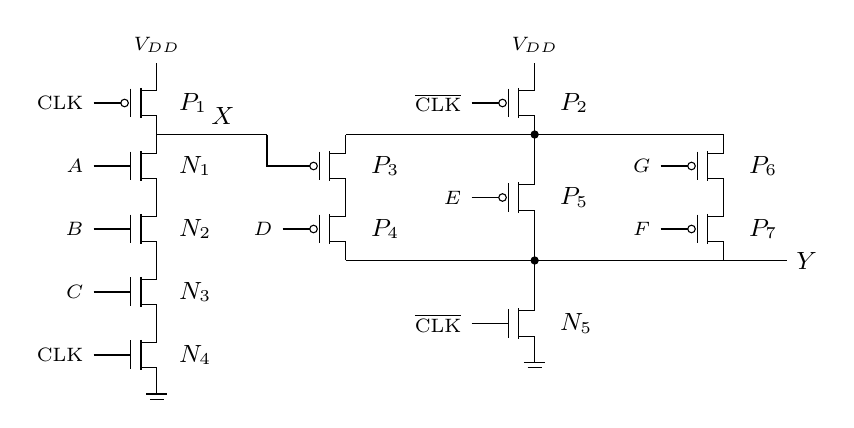
\begin{tikzpicture}[x=.8cm,y=.8cm,font=\small]
\mos{0}{6}{\mathrm{CLK}}{1}\rail{.25}{6.5}{V_{DD}}\mos{0}{5}{A}{0}\mos{0}{4}{B}{0}\mos{0}{3}{C}{0}\mos{0}{2}{\mathrm{CLK}}{0}\ground{.25}{1.5}
\draw(.25,5.5)--(2,5.5)node[above,pos=.6]{$X$};\node[right]at(.45,6){$P_1$};\node[right]at(.45,5){$N_1$};\node[right]at(.45,4){$N_2$};\node[right]at(.45,3){$N_3$};\node[right]at(.45,2){$N_4$};
\mos{6}{6}{\overline{\mathrm{CLK}}}{1}\rail{6.25}{6.5}{V_{DD}}
\draw(3.25,5.5)--(9.25,5.5);\fill(6.25,5.5)circle(1.5pt);\node[right]at(6.5,6){$P_2$};
\mos{3}{5}{}{1}\mos{3}{4}{D}{1}\mos{6}{4.5}{E}{1}\mos{9}{5}{G}{1}\mos{9}{4}{F}{1}
\draw(6.25,5)--(6.25,5.5);\draw(6.25,4)--(6.25,3.5);\draw(3.25,3.5)--(10.25,3.5)node[right]{$Y$};\fill(6.25,3.5)circle(1.5pt);
\draw(2,5.5)--(2,5)--(2.25,5);\node[right]at(3.5,5){$P_3$};\node[right]at(3.5,4){$P_4$};\node[right]at(6.5,4.5){$P_5$};\node[right]at(9.5,5){$P_6$};\node[right]at(9.5,4){$P_7$};
\mos{6}{2.5}{\overline{\mathrm{CLK}}}{0}\draw(6.25,3)--(6.25,3.5);\ground{6.25}{2}\node[right]at(6.5,2.5){$N_5$};
\end{tikzpicture}\\\small Figure 3: An NP-domino logic gate.\end{center}
\textbf{(a)} During precharge ($\mathrm{CLK}=0$), $X=1$ and $Y=0$. During evaluation, the left n-stack discharges $X$ for $ABC=1$. The right p-network charges $Y$ through a common header if $\bar X\bar D$, $\bar E$, or $\bar G\bar F$ is true:
\[\boxed{X=\overline{ABC},\qquad Y=ABC\bar D+\bar E+\bar F\bar G.}\]
The primary inputs must be stable during evaluation. $X$ is allowed only to fall, enabling a monotonic rise of $Y$ in the p-type stage. The matching student's function has a wrong grouping/complement; its dimensions and clock power can still be checked independently.
\textbf{(b)} All lengths are 20 nm. Let $R=R_{N5}$ for the printed $W_{N5}=20$ nm. With the n/p strength ratio two, $R_{P1}=R/2$ at the printed $W_{P1}=80$ nm. Equal division of the four-device n-stack gives $R_{N1}=\cdots=R_{N4}=R/8$, or $W_N=160$ nm. For the right stage choose the header and each two-device branch member at $R/3$, and the single-device branch at $2R/3$:
\begin{center}\begin{tabular}{lll}\toprule Devices&$W/L$ (nm)&Normalized resistance\\\midrule
$P_1$ (given)&80/20&$1/2$\\$N_1,N_2,N_3,N_4$&160/20&$1/8$ each\\
$P_2,P_3,P_4,P_6,P_7$&120/20&$1/3$ each\\$P_5$&60/20&$2/3$\\$N_5$ (given)&20/20&1\\\bottomrule\end{tabular}\end{center}
Then every charging branch to $Y$ is $R$ and its reset path is $R$. At $X$, both main rise and fall paths are $R/2$. The equal-path RC conditions hold even when the two output loads differ.
There are other valid allocations. For a right header resistance $\rho R$, $0<\rho<1$,
\[W_{P2}=40/\rho,\quad W_{P3,P4,P6,P7}=80/(1-\rho),\quad W_{P5}=40/(1-\rho)\ \mathrm{nm}.\]
Our conventional choice is $\rho=1/3$; it agrees with the graded widths. These are resistance-only/effective-load sizing conditions, not a specified transistor-capacitance optimization.
\newpage
\textbf{(c)} Since $C=C_{g,N5}$ and every channel length is the same, direct clock-gate capacitance scales with width:
\[C_{g,P1}=4C,\quad C_{g,N4}=8C,\quad C_{g,P2}=6C,\quad C_{g,N5}=C.\]
Both phases charge their directly attached gates once per full clock cycle, so
\[\boxed{P_{clock}=(4+8+6+1)CV_{DD}^2f=19CV_{DD}^2f.}\]
Clock generation and wire capacitance are not given and are excluded. There is no extra $1/2$ in the full-cycle supply energy $CV^2$. For the nonunique family above (same left-stack allocation), the coefficient is $13+2/\rho$; 19 belongs to the declared balanced sizing. The graded 19C result is consistent.
\qheading{6. Literal symbolic-layout extraction (10 points)}
The drawing has ten poly columns crossing both active rows: \textbf{20 physical MOS}, comprising eight inverters and two transmission gates. Split poly in columns 2 and 6 forms the separately controlled p/n halves of the TGs. Columns 3 and 7 form local clock inverters; they are not mere clock wires. The continuous U-shaped poly in columns 4 and 8 joins both corresponding feedback diffusion contacts. The final inverter's gate strap ends before its separate $Y$ drain strap.
\begin{center}\begin{tabular}{clll}\toprule Column&Devices&Gate(s)&Connected function\\\midrule
1&$I1P,I1N$&$X$&$a=\bar X$\\
2&$TGM\_P,TGM\_N$&$c_1,\mathrm{CLK}$&$a\leftrightarrow b$\\
3&$C1P,C1N$&$\mathrm{CLK}$&$c_1=\overline{\mathrm{CLK}}$\\
4&$M1P,M1N$&$b$&$m=\bar b$\\
5&$MFP,MFN$&$m$&$b=\bar m$, permanent feedback\\
6&$TGS\_P,TGS\_N$&$c_2,\overline{\mathrm{CLK}}$&$m\leftrightarrow d$\\
7&$C2P,C2N$&$\overline{\mathrm{CLK}}$&$c_2=\mathrm{CLK}$\\
8&$S1P,S1N$&$d$&$s=\bar d$\\
9&$SFP,SFN$&$s$&$d=\bar s$, permanent feedback\\
10&$O1P,O1N$&$s$&$Y=\bar s$\\\bottomrule\end{tabular}\end{center}
The upper diffusion is pMOS in n-well; conventional body connections are $V_{DD}$ for pMOS and $V_{SS}$ for nMOS. The source does not separately specify body-tap spacing or write strengths.
\newpage
\begin{center}\begin{tikzpicture}[x=0.72cm,y=0.72cm,font=\scriptsize]
\mos{0.0}{0.0}{X}{1}
\draw(0.25,0.5)--(0.25,0.75)node[above]{$ a $};
\draw(0.25,-0.5)--(0.25,-0.75)node[below]{$ V_{DD} $};
\node[anchor=west]at(0.55,0.0){\texttt{I1P}};
\mos{4.8}{0.0}{X}{0}
\draw(5.05,0.5)--(5.05,0.75)node[above]{$ a $};
\draw(5.05,-0.5)--(5.05,-0.75)node[below]{$ V_{SS} $};
\node[anchor=west]at(5.35,0.0){\texttt{I1N}};
\mos{9.6}{0.0}{\mathrm{c1}}{1}
\draw(9.85,0.5)--(9.85,0.75)node[above]{$ b $};
\draw(9.85,-0.5)--(9.85,-0.75)node[below]{$ a $};
\node[anchor=west]at(10.15,0.0){\texttt{TGM\_P}};
\mos{14.399999999999999}{0.0}{\mathrm{CLK}}{0}
\draw(14.649999999999999,0.5)--(14.649999999999999,0.75)node[above]{$ b $};
\draw(14.649999999999999,-0.5)--(14.649999999999999,-0.75)node[below]{$ a $};
\node[anchor=west]at(14.95,0.0){\texttt{TGM\_N}};
\mos{0.0}{-2.8}{\mathrm{CLK}}{1}
\draw(0.25,-2.3)--(0.25,-2.05)node[above]{$ \mathrm{c1} $};
\draw(0.25,-3.3)--(0.25,-3.55)node[below]{$ V_{DD} $};
\node[anchor=west]at(0.55,-2.8){\texttt{C1P}};
\mos{4.8}{-2.8}{\mathrm{CLK}}{0}
\draw(5.05,-2.3)--(5.05,-2.05)node[above]{$ \mathrm{c1} $};
\draw(5.05,-3.3)--(5.05,-3.55)node[below]{$ V_{SS} $};
\node[anchor=west]at(5.35,-2.8){\texttt{C1N}};
\mos{9.6}{-2.8}{b}{1}
\draw(9.85,-2.3)--(9.85,-2.05)node[above]{$ m $};
\draw(9.85,-3.3)--(9.85,-3.55)node[below]{$ V_{DD} $};
\node[anchor=west]at(10.15,-2.8){\texttt{M1P}};
\mos{14.399999999999999}{-2.8}{b}{0}
\draw(14.649999999999999,-2.3)--(14.649999999999999,-2.05)node[above]{$ m $};
\draw(14.649999999999999,-3.3)--(14.649999999999999,-3.55)node[below]{$ V_{SS} $};
\node[anchor=west]at(14.95,-2.8){\texttt{M1N}};
\mos{0.0}{-5.6}{m}{1}
\draw(0.25,-5.1)--(0.25,-4.85)node[above]{$ b $};
\draw(0.25,-6.1)--(0.25,-6.35)node[below]{$ V_{DD} $};
\node[anchor=west]at(0.55,-5.6){\texttt{MFP}};
\mos{4.8}{-5.6}{m}{0}
\draw(5.05,-5.1)--(5.05,-4.85)node[above]{$ b $};
\draw(5.05,-6.1)--(5.05,-6.35)node[below]{$ V_{SS} $};
\node[anchor=west]at(5.35,-5.6){\texttt{MFN}};
\mos{9.6}{-5.6}{\mathrm{c2}}{1}
\draw(9.85,-5.1)--(9.85,-4.85)node[above]{$ d $};
\draw(9.85,-6.1)--(9.85,-6.35)node[below]{$ m $};
\node[anchor=west]at(10.15,-5.6){\texttt{TGS\_P}};
\mos{14.399999999999999}{-5.6}{\overline{\mathrm{CLK}}}{0}
\draw(14.649999999999999,-5.1)--(14.649999999999999,-4.85)node[above]{$ d $};
\draw(14.649999999999999,-6.1)--(14.649999999999999,-6.35)node[below]{$ m $};
\node[anchor=west]at(14.95,-5.6){\texttt{TGS\_N}};
\mos{0.0}{-8.399999999999999}{\overline{\mathrm{CLK}}}{1}
\draw(0.25,-7.899999999999999)--(0.25,-7.649999999999999)node[above]{$ \mathrm{c2} $};
\draw(0.25,-8.899999999999999)--(0.25,-9.149999999999999)node[below]{$ V_{DD} $};
\node[anchor=west]at(0.55,-8.399999999999999){\texttt{C2P}};
\mos{4.8}{-8.399999999999999}{\overline{\mathrm{CLK}}}{0}
\draw(5.05,-7.899999999999999)--(5.05,-7.649999999999999)node[above]{$ \mathrm{c2} $};
\draw(5.05,-8.899999999999999)--(5.05,-9.149999999999999)node[below]{$ V_{SS} $};
\node[anchor=west]at(5.35,-8.399999999999999){\texttt{C2N}};
\mos{9.6}{-8.399999999999999}{d}{1}
\draw(9.85,-7.899999999999999)--(9.85,-7.649999999999999)node[above]{$ s $};
\draw(9.85,-8.899999999999999)--(9.85,-9.149999999999999)node[below]{$ V_{DD} $};
\node[anchor=west]at(10.15,-8.399999999999999){\texttt{S1P}};
\mos{14.399999999999999}{-8.399999999999999}{d}{0}
\draw(14.649999999999999,-7.899999999999999)--(14.649999999999999,-7.649999999999999)node[above]{$ s $};
\draw(14.649999999999999,-8.899999999999999)--(14.649999999999999,-9.149999999999999)node[below]{$ V_{SS} $};
\node[anchor=west]at(14.95,-8.399999999999999){\texttt{S1N}};
\mos{0.0}{-11.2}{s}{1}
\draw(0.25,-10.7)--(0.25,-10.45)node[above]{$ d $};
\draw(0.25,-11.7)--(0.25,-11.95)node[below]{$ V_{DD} $};
\node[anchor=west]at(0.55,-11.2){\texttt{SFP}};
\mos{4.8}{-11.2}{s}{0}
\draw(5.05,-10.7)--(5.05,-10.45)node[above]{$ d $};
\draw(5.05,-11.7)--(5.05,-11.95)node[below]{$ V_{SS} $};
\node[anchor=west]at(5.35,-11.2){\texttt{SFN}};
\mos{9.6}{-11.2}{s}{1}
\draw(9.85,-10.7)--(9.85,-10.45)node[above]{$ Y $};
\draw(9.85,-11.7)--(9.85,-11.95)node[below]{$ V_{DD} $};
\node[anchor=west]at(10.15,-11.2){\texttt{O1P}};
\mos{14.399999999999999}{-11.2}{s}{0}
\draw(14.649999999999999,-10.7)--(14.649999999999999,-10.45)node[above]{$ Y $};
\draw(14.649999999999999,-11.7)--(14.649999999999999,-11.95)node[below]{$ V_{SS} $};
\node[anchor=west]at(14.95,-11.2){\texttt{O1N}};
\end{tikzpicture}\end{center}
\small All 20 physical devices, in source column order. A TG is bidirectional; its drain/source naming is a netlist convention. Identically named terminals are connected. All nMOS bodies use $V_{SS}$; all pMOS bodies use $V_{DD}$.\normalsize\par
When CLK is high, the first TG is on and the second is off; when CLK falls, the first closes and the second opens. Thus the structure is \emph{conditionally} a falling-edge register with $Y=X$. The feedback inverters in columns 5 and 9 remain permanently attached. During an attempted write against old state, their drive contends with the incoming value. A ratio/analog condition is needed for the input to win; no widths are given, so a guaranteed writeable latch cannot be asserted from connectivity alone.
The verifier enumerates 16 settled/write-attempt switch states, including the contending cases, and 24 conditional edge events. It does not replace the source with a conventional two-TG latch or silently disconnect feedback.
\textbf{Source comparison.} This question is absent from the supplied graded booklet. A similar later-year layout was used only to cross-check a contact graph first traced from this year's full native photograph; all 20 crossings, local clock inverters and feedback joins were confirmed directly.
\newpage
\qheading{7. Master latch and low-cost slave (10 points)}
\textbf{(a)} In the following figure, the upper control is the pMOS gate and the lower control is the nMOS gate. The master input TG is on for CLK=1. The master feedback TG and slave input TG are on for CLK=0. Therefore the master closes and slave opens at the falling edge.
\begin{center}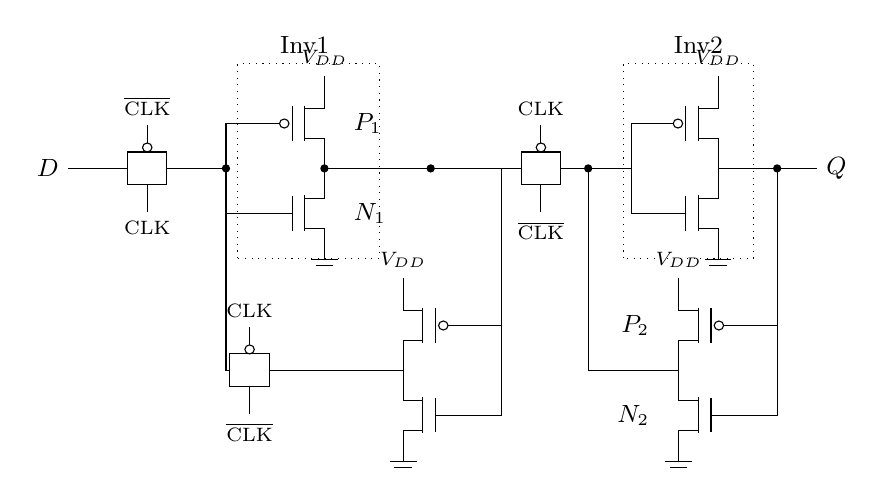
\begin{tikzpicture}[x=1cm,y=.95cm,font=\small]
\tg{1}{4.1}{\overline{\mathrm{CLK}}}{\mathrm{CLK}}\tg{2.3}{1.4}{\mathrm{CLK}}{\overline{\mathrm{CLK}}}\tg{6}{4.1}{\mathrm{CLK}}{\overline{\mathrm{CLK}}}
\draw(0,4.1)--(.75,4.1)node[pos=0,left]{$D$};\draw(1.25,4.1)--(2,4.1);\draw(2,3.5)--(2,4.7)--(2.25,4.7);\draw(2,3.5)--(2.25,3.5);\fill(2,4.1)circle(1.5pt);
\mos{3}{4.7}{}{1}\mos{3}{3.5}{}{0}\rail{3.25}{5.2}{V_{DD}}\ground{3.25}{3}\draw(3.25,4.0)--(3.25,4.2);\draw(3.25,4.1)--(5.75,4.1);\fill(3.25,4.1)circle(1.5pt);
\node[right]at(3.5,4.7){$P_1$};\node[right]at(3.5,3.5){$N_1$};\draw[dotted](2.15,2.9)rectangle(3.95,5.5);\node[above]at(3,5.5){Inv1};
\mosR{4.5}{2}{}{1}\mosR{4.5}{.8}{}{0}\rail{4.25}{2.5}{V_{DD}}\ground{4.25}{.3}\draw(4.25,1.3)--(4.25,1.5);\draw(4.25,1.4)--(2.55,1.4);\draw(2.05,1.4)--(2,1.4)--(2,4.1);
\draw(4.6,4.1)--(5.5,4.1)--(5.5,.8)--(5.25,.8);\draw(5.5,2)--(5.25,2);\fill(4.6,4.1)circle(1.5pt);
\draw(6.25,4.1)--(6.6,4.1);\draw(6.6,4.1)--(7.15,4.1)--(7.15,4.7)--(7.25,4.7);\draw(7.15,4.1)--(7.15,3.5)--(7.25,3.5);\fill(6.6,4.1)circle(1.5pt);
\mos{8}{4.7}{}{1}\mos{8}{3.5}{}{0}\rail{8.25}{5.2}{V_{DD}}\ground{8.25}{3}\draw(8.25,4)--(8.25,4.2);\draw(8.25,4.1)--(9.5,4.1)node[right]{$Q$};
\draw[dotted](7.05,2.9)rectangle(8.7,5.5);\node[above]at(8,5.5){Inv2};
\mosR{8}{2}{}{1}\mosR{8}{.8}{}{0}\rail{7.75}{2.5}{V_{DD}}\ground{7.75}{.3}\draw(7.75,1.3)--(7.75,1.5);\draw(7.75,1.4)--(6.6,1.4)--(6.6,4.1);
\draw(9,4.1)--(9,.8)--(8.75,.8);\draw(9,2)--(8.75,2);\fill(9,4.1)circle(1.5pt);\node[left]at(7.5,2){$P_2$};\node[left]at(7.5,.8){$N_2$};
\end{tikzpicture}\\\small Figure 5: A static register. Clock labels filled for falling-edge operation.\end{center}
There are 14 MOS: master 2TG+2INV (8), slave 1TG+2INV (6). The slave feedback inverter $P_2/N_2$ is permanently connected, as in the original.
\textbf{(b)} With the stated classroom forward-settling convention,
\[\boxed{t_{setup}=t_{TG}+t_{Inv1}=0.10+0.15=0.25\ \mathrm{ns}.}\]
Inv2 is after the closing master latch and contributes to clock-to-output delay, not this setup sum. The analogous forward clock-to-Q estimate is $0.10+0.20=0.30$ ns. Full transistor-level setup characterization also depends on feedback, clock overlap and analog switching, which are not supplied.
\textbf{(c)} To overwrite slave feedback when the new master output is high, the old $N_2$ pull-down must lose:
\[\frac{V_{DD}R_{N2}}{R_{P1}+R_{TS}+R_{N2}}>\frac{V_{DD}}2
\quad\Longrightarrow\quad\boxed{R_{N2}>R_{P1}+R_{TS}.}\]
To write low against the old $P_2$ pull-up,
\[\frac{V_{DD}(R_{N1}+R_{TS})}{R_{P2}+R_{N1}+R_{TS}}<\frac{V_{DD}}2
\quad\Longrightarrow\quad\boxed{R_{P2}>R_{N1}+R_{TS}.}\]
Strict inequalities provide crossing margin. They make the slave feedback weaker than the complete forward master-plus-TG path. Equal-strength feedback or ignoring the TG resistance can prevent a write. This question is not present in the supplied graded booklet; the result comes from the original circuit and the stated $V_{DD}/2$ threshold.
\newpage
\qheading{8. Hold repair, frequency and aligned pipeline (15 points)}
Let $q_i$ denote the outputs of R1--R3. The printed gates give
\[u=q_1\odot q_2,\quad v=\bar u,\quad p=q_2q_3,\quad r=vq_3,\]
\[Y_1=q_3,\qquad Y_2=p+r=q_3(q_1+q_2),\qquad Y_3=u\odot q_3=q_1\oplus q_2\oplus q_3.\]
Here $\odot$ is XNOR. Simplification checks functionality; timing is evaluated on the printed physical gate paths.
\textbf{(a) The direct R3$\to$R4 path violates hold.}
\[t_{ccq}+t_{cd,logic}=0.1+0<0.2=t_{hold}.\]
Increasing the clock period does not repair same-edge hold. First method: insert two inverters only on the R3-to-R4 branch. They preserve $Y_1$ polarity and add the printed $0.4$ ns propagation delay, without lengthening the critical Y2 path.
\begin{center}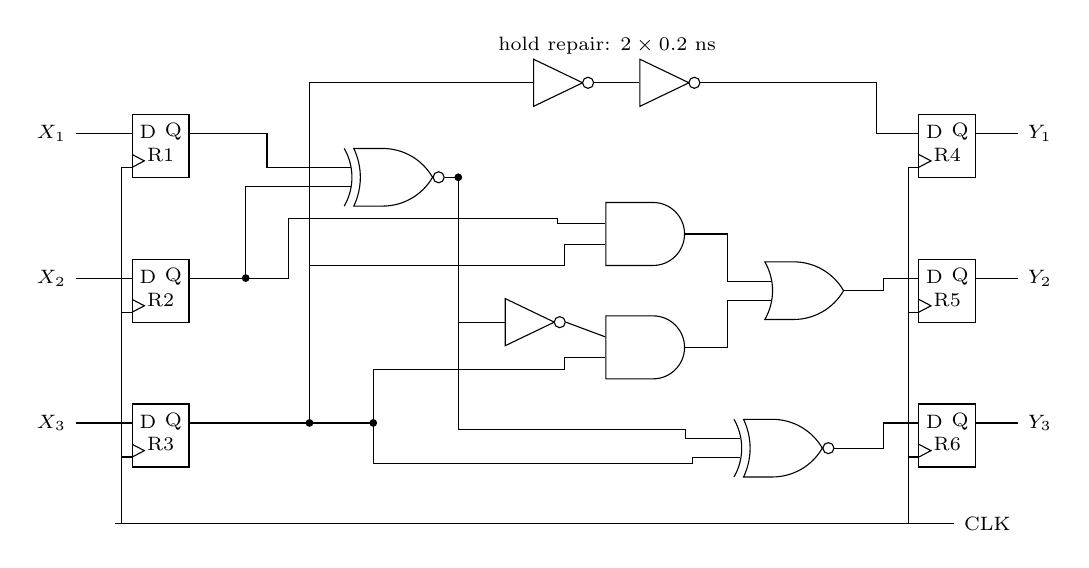
\begin{tikzpicture}[x=.9cm,y=.8cm,font=\scriptsize]
\draw(-0.4,5.5)rectangle(0.4,6.5);\node at(0,5.86){R1};\node at(-0.18,6.22){D};\node at(0.18,6.22){Q};\draw(-0.4,5.66)--(-0.23,5.76)--(-0.4,5.86);
\draw(10.7,5.5)rectangle(11.5,6.5);\node at(11.1,5.86){R4};\node at(10.92,6.22){D};\node at(11.28,6.22){Q};\draw(10.7,5.66)--(10.87,5.76)--(10.7,5.86);
\draw(-1.2,6.2)--(-.4,6.2)node[pos=0,left]{$X_1$};\draw(11.5,6.2)--(12.1,6.2)node[right]{$Y_1$};
\draw(-0.4,3.2)rectangle(0.4,4.2);\node at(0,3.56){R2};\node at(-0.18,3.9200000000000004){D};\node at(0.18,3.9200000000000004){Q};\draw(-0.4,3.3600000000000003)--(-0.23,3.46)--(-0.4,3.56);
\draw(10.7,3.2)rectangle(11.5,4.2);\node at(11.1,3.56){R5};\node at(10.92,3.9200000000000004){D};\node at(11.28,3.9200000000000004){Q};\draw(10.7,3.3600000000000003)--(10.87,3.46)--(10.7,3.56);
\draw(-1.2,3.9000000000000004)--(-.4,3.9000000000000004)node[pos=0,left]{$X_2$};\draw(11.5,3.9000000000000004)--(12.1,3.9000000000000004)node[right]{$Y_2$};
\draw(-0.4,0.8999999999999999)rectangle(0.4,1.9);\node at(0,1.2599999999999998){R3};\node at(-0.18,1.6199999999999999){D};\node at(0.18,1.6199999999999999){Q};\draw(-0.4,1.0599999999999998)--(-0.23,1.16)--(-0.4,1.2599999999999998);
\draw(10.7,0.8999999999999999)rectangle(11.5,1.9);\node at(11.1,1.2599999999999998){R6};\node at(10.92,1.6199999999999999){D};\node at(11.28,1.6199999999999999){Q};\draw(10.7,1.0599999999999998)--(10.87,1.16)--(10.7,1.2599999999999998);
\draw(-1.2,1.5999999999999999)--(-.4,1.5999999999999999)node[pos=0,left]{$X_3$};\draw(11.5,1.5999999999999999)--(12.1,1.5999999999999999)node[right]{$Y_3$};
\node[xnor gate US,draw,logic gate inputs=nn,minimum width=1cm](u)at(3.2,5.5){};
\draw(.4,6.2)--(1.5,6.2)|-(u.input 1);\draw(.4,3.9)--(1.2,3.9)|-(u.input 2);
\node[not gate US,draw,minimum width=.7cm](v)at(5.1,3.2){};
\draw(u.output)--(4.2,5.5)--(4.2,3.2)--(v.input);\fill(4.2,5.5)circle(1.4pt);
\node[and gate US,draw,logic gate inputs=nn,minimum width=1cm](p)at(6.8,4.6){};\node[and gate US,draw,logic gate inputs=nn,minimum width=1cm](r)at(6.8,2.8){};
\draw(1.2,3.9)--(1.8,3.9)--(1.8,4.85)--(5.6,4.85)|-(p.input 1);\fill(1.2,3.9)circle(1.4pt);
\draw(.4,1.6)--(2.1,1.6)--(2.1,4.1)--(5.7,4.1)|-(p.input 2);\fill(2.1,1.6)circle(1.4pt);
\draw(v.output)--(r.input 1);\draw(2.1,1.6)--(3,1.6)--(3,2.45)--(5.7,2.45)|-(r.input 2);\fill(3,1.6)circle(1.4pt);
\node[or gate US,draw,logic gate inputs=nn,minimum width=1cm](o)at(9,3.7){};\draw(p.output)--(8,4.6)|-(o.input 1);\draw(r.output)--(8,2.8)|-(o.input 2);\draw(o.output)--(10.2,3.7)|-(10.7,3.9);
\node[xnor gate US,draw,logic gate inputs=nn,minimum width=1cm](z)at(8.7,1.2){};\draw(4.2,5.5)--(4.2,1.5)--(7.4,1.5)|-(z.input 1);\draw(3,1.6)--(3,.95)--(7.5,.95)|-(z.input 2);\draw(z.output)--(10.2,1.2)|-(10.7,1.6);
\node[not gate US,draw,minimum width=.7cm](b1)at(5.5,7){};\node[not gate US,draw,minimum width=.7cm](b2)at(7,7){};\draw(2.1,4.1)--(2.1,7)--(b1.input);\draw(b1.output)--(b2.input);\draw(b2.output)--(10.1,7)|-(10.7,6.2);\node[above]at(6.3,7.3){hold repair: $2\times0.2$ ns};
\draw(-.65,0)--(11.2,0)node[right]{$\mathrm{CLK}$};\foreach\x in {-.55,10.55}{\foreach\y in {5.66,3.36,1.06}{\draw(\x,0)--(\x,\y)--++(.15,0);}}
\end{tikzpicture}\end{center}
The real requirement is $t_{cd,buffers}\ge0.1$ ns and $t_{pd,buffers}\le1.6$ ns. If the classroom model treats the two printed inverter delays as minimum as well as maximum, the pair satisfies both. Propagation delay alone is not proof of contamination delay; the conditional requirement is stated explicitly.
\newpage
\textbf{Second method: a low-level transparent lockup latch only on the direct branch.}
\begin{center}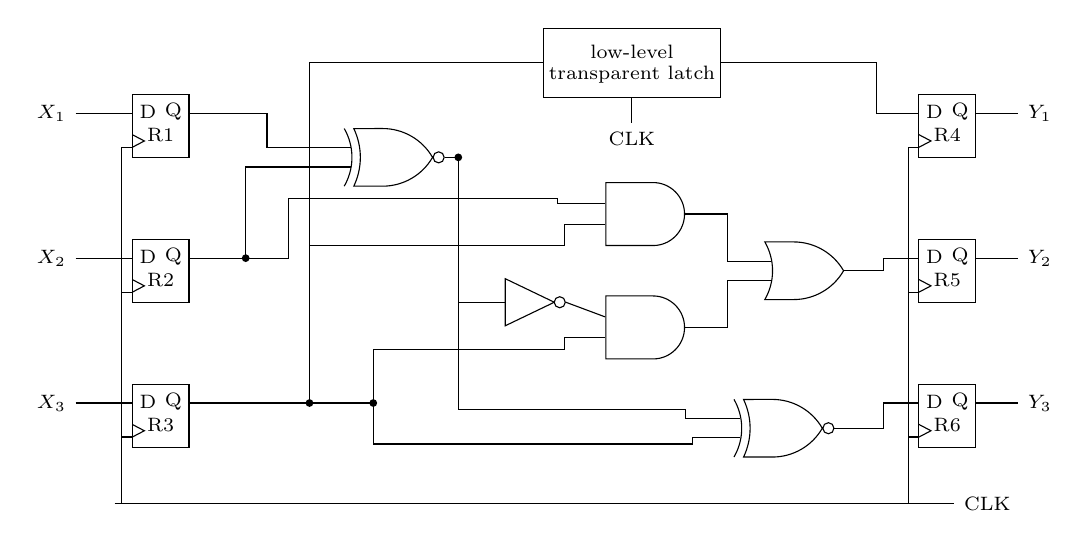
\begin{tikzpicture}[x=.9cm,y=.8cm,font=\scriptsize]
\draw(-0.4,5.5)rectangle(0.4,6.5);\node at(0,5.86){R1};\node at(-0.18,6.22){D};\node at(0.18,6.22){Q};\draw(-0.4,5.66)--(-0.23,5.76)--(-0.4,5.86);
\draw(10.7,5.5)rectangle(11.5,6.5);\node at(11.1,5.86){R4};\node at(10.92,6.22){D};\node at(11.28,6.22){Q};\draw(10.7,5.66)--(10.87,5.76)--(10.7,5.86);
\draw(-1.2,6.2)--(-.4,6.2)node[pos=0,left]{$X_1$};\draw(11.5,6.2)--(12.1,6.2)node[right]{$Y_1$};
\draw(-0.4,3.2)rectangle(0.4,4.2);\node at(0,3.56){R2};\node at(-0.18,3.9200000000000004){D};\node at(0.18,3.9200000000000004){Q};\draw(-0.4,3.3600000000000003)--(-0.23,3.46)--(-0.4,3.56);
\draw(10.7,3.2)rectangle(11.5,4.2);\node at(11.1,3.56){R5};\node at(10.92,3.9200000000000004){D};\node at(11.28,3.9200000000000004){Q};\draw(10.7,3.3600000000000003)--(10.87,3.46)--(10.7,3.56);
\draw(-1.2,3.9000000000000004)--(-.4,3.9000000000000004)node[pos=0,left]{$X_2$};\draw(11.5,3.9000000000000004)--(12.1,3.9000000000000004)node[right]{$Y_2$};
\draw(-0.4,0.8999999999999999)rectangle(0.4,1.9);\node at(0,1.2599999999999998){R3};\node at(-0.18,1.6199999999999999){D};\node at(0.18,1.6199999999999999){Q};\draw(-0.4,1.0599999999999998)--(-0.23,1.16)--(-0.4,1.2599999999999998);
\draw(10.7,0.8999999999999999)rectangle(11.5,1.9);\node at(11.1,1.2599999999999998){R6};\node at(10.92,1.6199999999999999){D};\node at(11.28,1.6199999999999999){Q};\draw(10.7,1.0599999999999998)--(10.87,1.16)--(10.7,1.2599999999999998);
\draw(-1.2,1.5999999999999999)--(-.4,1.5999999999999999)node[pos=0,left]{$X_3$};\draw(11.5,1.5999999999999999)--(12.1,1.5999999999999999)node[right]{$Y_3$};
\node[xnor gate US,draw,logic gate inputs=nn,minimum width=1cm](u)at(3.2,5.5){};
\draw(.4,6.2)--(1.5,6.2)|-(u.input 1);\draw(.4,3.9)--(1.2,3.9)|-(u.input 2);
\node[not gate US,draw,minimum width=.7cm](v)at(5.1,3.2){};
\draw(u.output)--(4.2,5.5)--(4.2,3.2)--(v.input);\fill(4.2,5.5)circle(1.4pt);
\node[and gate US,draw,logic gate inputs=nn,minimum width=1cm](p)at(6.8,4.6){};\node[and gate US,draw,logic gate inputs=nn,minimum width=1cm](r)at(6.8,2.8){};
\draw(1.2,3.9)--(1.8,3.9)--(1.8,4.85)--(5.6,4.85)|-(p.input 1);\fill(1.2,3.9)circle(1.4pt);
\draw(.4,1.6)--(2.1,1.6)--(2.1,4.1)--(5.7,4.1)|-(p.input 2);\fill(2.1,1.6)circle(1.4pt);
\draw(v.output)--(r.input 1);\draw(2.1,1.6)--(3,1.6)--(3,2.45)--(5.7,2.45)|-(r.input 2);\fill(3,1.6)circle(1.4pt);
\node[or gate US,draw,logic gate inputs=nn,minimum width=1cm](o)at(9,3.7){};\draw(p.output)--(8,4.6)|-(o.input 1);\draw(r.output)--(8,2.8)|-(o.input 2);\draw(o.output)--(10.2,3.7)|-(10.7,3.9);
\node[xnor gate US,draw,logic gate inputs=nn,minimum width=1cm](z)at(8.7,1.2){};\draw(4.2,5.5)--(4.2,1.5)--(7.4,1.5)|-(z.input 1);\draw(3,1.6)--(3,.95)--(7.5,.95)|-(z.input 2);\draw(z.output)--(10.2,1.2)|-(10.7,1.6);
\draw(2.1,4.1)--(2.1,7)--(5.4,7);\draw(5.4,6.45)rectangle(7.9,7.55);\node at(6.65,7.18){low-level};\node at(6.65,6.82){transparent latch};\draw(7.9,7)--(10.1,7)|-(10.7,6.2);\draw(6.65,6.45)--(6.65,6.05)node[below]{$\mathrm{CLK}$};
\draw(-.65,0)--(11.2,0)node[right]{$\mathrm{CLK}$};\foreach\x in {-.55,10.55}{\foreach\y in {5.66,3.36,1.06}{\draw(\x,0)--(\x,\y)--++(.15,0);}}
\end{tikzpicture}\end{center}
This latch closes at the launch rising edge, retains the previous value through the high phase, and opens after the falling edge. Let high time be $H$ and low time $T-H$; let its delays/setup/hold be $t_{pd,L},t_{cd,L},t_{setup,L},t_{hold,L}$. Sufficient zero-skew timing conditions are
\[H\ge0.2,\quad T-H\ge t_{pd,L}+0.2,\quad H+t_{cd,L}\ge0.2,\]
\[t_{hold,L}\le0.1,\qquad t_{setup,L}\le T-0.2.\]
At $T=2$ ns and 50\% duty, an explicitly ideal latch satisfies these; a nonideal latch needs, in particular, $t_{pd,L}\le0.8$ ns plus the other bounds. The paper gives no latch parameters or duty for this alternative, so it is a conditional design rather than an invented numerical guarantee.
\textbf{(b) Repaired maximum frequency: $\boxed{500\ \mathrm{MHz}}$.}
The longest path to R5 is XNOR$\to$INV$\to$AND$\to$OR:
\[t_{pd,max}=0.4+0.2+0.5+0.5=1.6\ \mathrm{ns},\quad T_{min}=0.2+1.6+0.2=2.0\ \mathrm{ns}.\]
The two-inverter direct repair has setup requirement only $0.2+0.4+0.2=0.8$ ns. The student's 2 ns/full-credit frequency agrees with the independent calculation; this does not certify its separate hold solution.
\textbf{(c) Target is $4/3$, not four, times the original frequency.}
\[f_{target}=\frac43(500)=666.\overline6\ \mathrm{MHz},\quad T_{target}=1.5\ \mathrm{ns},\quad t_{logic,budget}=1.5-0.2-0.2=1.1\ \mathrm{ns}.\]
A bare period calculation is insufficient: reconvergent signals and all three outputs must be delayed by the same added cycle.
\newpage
Insert four registers after $p,r,u,q_3$, respectively. Include one two-inverter hold pair before the $q_3$ cut register and a \emph{separate} pair from it to R4:
\begin{center}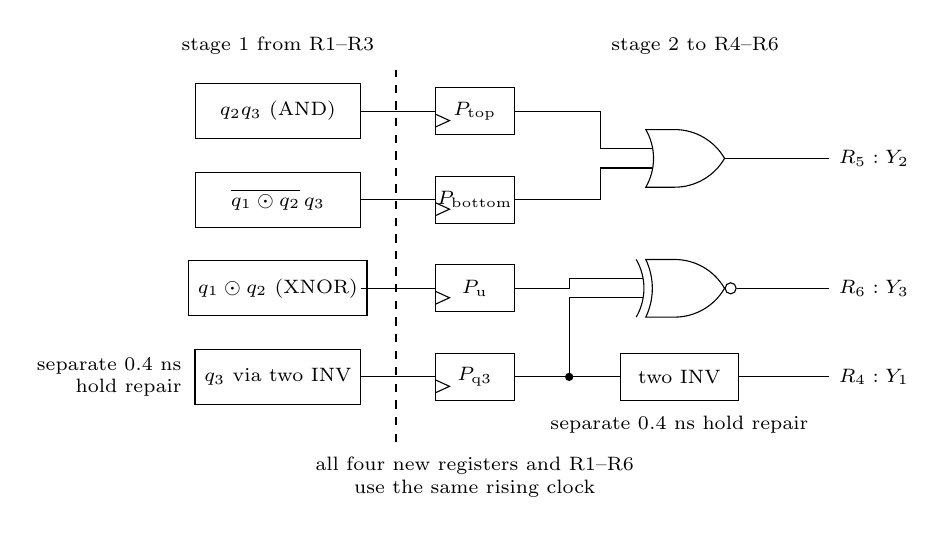
\begin{tikzpicture}[x=1cm,y=.75cm,font=\scriptsize]
\node[draw,minimum width=2.1cm,minimum height=.7cm](a)at(0,5){$q_2q_3$ (AND)};
\node[draw,minimum width=2.1cm,minimum height=.7cm](b)at(0,3.5){$\overline{q_1\odot q_2}\,q_3$};
\node[draw,minimum width=2.1cm,minimum height=.7cm](c)at(0,2){$q_1\odot q_2$ (XNOR)};
\node[draw,minimum width=2.1cm,minimum height=.7cm](d)at(0,.5){$q_3$ via two INV};
\foreach\y/\n in {5/top,3.5/bottom,2/u,.5/q3}{\draw(2,\y-.4)rectangle(3,\y+.4);\node at(2.5,\y){$P_{\mathrm{\n}}$};\draw(1.05,\y)--(2,\y);\draw(2,\y-.27)--(2.18,\y-.16)--(2,\y-.05);}
\node[or gate US,draw,logic gate inputs=nn,minimum width=1cm](o)at(5.1,4.2){};\draw(3,5)--(4.1,5)|-(o.input 1);\draw(3,3.5)--(4.1,3.5)|-(o.input 2);\draw(o.output)--(7,4.2)node[right]{$R_5:Y_2$};
\node[xnor gate US,draw,logic gate inputs=nn,minimum width=1cm](z)at(5.1,2){};\draw(3,2)--(3.7,2)|-(z.input 1);\draw(3,.5)--(3.7,.5)--(3.7,1.7)|-(z.input 2);\fill(3.7,.5)circle(1.5pt);\draw(z.output)--(7,2)node[right]{$R_6:Y_3$};
\node[draw,minimum width=1.5cm,minimum height=.6cm](h)at(5.1,.5){two INV};\draw(3.7,.5)--(h.west);\draw(h.east)--(7,.5)node[right]{$R_4:Y_1$};
\draw[dashed](1.5,-.6)--(1.5,5.7);\node[above]at(0,5.8){stage 1 from R1--R3};\node[above]at(5.3,5.8){stage 2 to R4--R6};
\node[below,align=center]at(2.5,-.7){all four new registers and R1--R6\\use the same rising clock};
\node[left,align=right]at(-1.1,.5){separate $0.4$ ns\\hold repair};\node[below]at(5.1,0){separate $0.4$ ns hold repair};
\end{tikzpicture}\end{center}
\begin{center}\begin{tabular}{lll}\toprule Stage&Longest relevant gate sequence&Delay (ns)\\\midrule
1 to $P_{bottom}$&XNOR, INV, AND&1.1\\
1 to $P_{top}$&AND&0.5\\
1 to $P_u$&XNOR&0.4\\
1 to $P_{q3}$&INV, INV (hold repair)&0.4\\
2 to R5&OR&0.5\\
2 to R6&XNOR&0.4\\
2 to R4&INV, INV (separate hold repair)&0.4\\\bottomrule\end{tabular}\end{center}
The maximum setup requirement is $0.2+1.1+0.2=1.5$ ns, so the target is reached exactly in the stated model. The second stage combines stored $p,r,u,q_3$ from the same sample, adding one aligned cycle to all three outputs. Each new bypass path still requires actual logic contamination delay at least 0.1 ns; printed gate propagation values justify hold only under the classroom minimum-equals-maximum convention.
The verifier checks all eight input functions, every listed launch/capture path, and 64 consecutive two-sample combinations. The supplied answer contains the 1.5 ns/1.1 ns arithmetic but no completed aligned register cut; the diagram above supplies that missing design.
\qheading{Verification and source scope}
The saved CSVs contain 8 domino truth cases and 64 phase/node checks; 16 complex-function cases and 32 dynamic phase checks; 128 NP input cases and 512 phase/node checks; 16 literal-layout and 16 low-cost-register switch states; 24 conditional layout edge events; and 64 consecutive pipeline sample pairs. Sizing/leakage/timing use analytical equations and exact rational arithmetic where appropriate. Analog DSL bias and ratioed writeability are explicitly outside ideal rail verification.
The prompt comes from the first three Fall 2018 pages of the supplied loose PDF, cross-checked with the ZIP's three original pages (ZIP footer order F-3,F-1,F-2). The four-page graded booklet is a fallible reference; its identity pages remain local. The authoritative DSL topology reference is Li, \href{https://www.ee.ncu.edu.tw/jfli/public_html/VLSI/lecture/ch06.pdf}{Chapter 6 lecture, slide 32}. The README summarizes question coverage and the independent analytical checks.
\end{document}
